%==============================================================================
% ETH Zurich -- 3D Vision poster  (A1, portrait)
% Light theme: light-grey page, white rounded cards, ETH-blue accents.
% Compiles with pdflatex (two passes).
%==============================================================================
\documentclass[final]{beamer}
\usepackage[orientation=portrait,size=a1,scale=1.0]{beamerposter}

\usepackage[utf8]{inputenc}
\usepackage[T1]{fontenc}
\usepackage{helvet}
\renewcommand{\familydefault}{\sfdefault}
\usepackage{graphicx}
\usepackage{booktabs}
\usepackage{amsmath}
\usepackage{tikz}
\usetikzlibrary{arrows.meta,positioning,shapes.geometric,calc}
\usepackage{pgfplots}
\pgfplotsset{compat=1.16}
\usepackage{xcolor}

%------------------------------------------------------------------ colours
\definecolor{ETHBlue}{HTML}{215CAF}
\definecolor{ETHBlueDark}{HTML}{123362}
\definecolor{BlueTint}{HTML}{E7EEF8}
\definecolor{ETHPetrol}{HTML}{007894}
\definecolor{PageBg}{HTML}{EAEBEE}     % light cool-grey page
\definecolor{CardEdge}{HTML}{DEE0E4}
\definecolor{ETHText}{HTML}{1A1A1A}
\definecolor{ETHGrey}{HTML}{6F6F6F}
\definecolor{ETHCaption}{HTML}{707070}
\definecolor{BarGray}{HTML}{A6ABB2}    % baseline bars
\definecolor{BarLite}{HTML}{C9CDD3}    % VGGT-only reference
\definecolor{GainPos}{HTML}{2E7D32}    % small positive accent for deltas

\colorlet{accent}{ETHBlue}

%------------------------------------------------------------------ geometry: even frame + gutter
\newlength{\margin}\setlength{\margin}{1.7cm}
\newlength{\gutter}\setlength{\gutter}{1.7cm}
\setbeamersize{text margin left=\margin,text margin right=\margin}
\setlength{\columnsep}{\gutter}
\newlength{\colwidth}
\setlength{\colwidth}{\dimexpr0.5\paperwidth-\margin-0.5\gutter\relax}
\newlength{\colheight}\setlength{\colheight}{63.0cm}
\newcommand{\flexgap}{\vspace{\gutter}\vfill}

%------------------------------------------------------------------ canvas
\usetheme{default}
\setbeamertemplate{navigation symbols}{}
\setbeamercolor{background canvas}{bg=PageBg}     % AFTER usetheme
\setbeamercolor{normal text}{fg=ETHText,bg=white}

%------------------------------------------------------------------ white rounded cards, blue-tint title strip
\setbeamertemplate{blocks}[rounded][shadow=false]
\setbeamercolor{block title}{fg=ETHBlueDark,bg=BlueTint}
\setbeamercolor{block body}{fg=ETHText,bg=white}
\setbeamerfont{block title}{series=\bfseries,size=\LARGE}
\setbeamerfont{block body}{size=\large}

% numbered sections: blue circled number + dark title, in the tinted strip
\newcounter{secno}
\newcommand{\secbadge}[1]{\tikz[baseline=(c.base)]{\node[circle,fill=ETHBlue,
  text=white,inner sep=0pt,minimum size=1.15em,font=\bfseries](c){#1};}}
\newenvironment{psection}[1]{%
  \stepcounter{secno}%
  \begin{block}{\secbadge{\thesecno}\hskip0.5em #1}%
}{\end{block}}

\setbeamertemplate{itemize item}{\color{accent}\raise0.12ex\hbox{\small$\blacksquare$}}
\setbeamertemplate{itemize subitem}{\color{accent}\raise0.1ex\hbox{\footnotesize$\bullet$}}
\setlength{\leftmargini}{1.4em}

\newcommand{\cpt}[1]{{\small\color{ETHCaption}#1}}

% shared pgfplots style for the result charts
\pgfplotsset{
  posterchart/.style={
    width=0.86\linewidth, height=10.5cm,
    axis lines=left, axis line style={ETHGrey!60},
    every tick label/.append style={font=\normalsize,color=ETHText},
    ymajorgrids, grid style={CardEdge},
    title style={font=\large\bfseries,color=ETHBlueDark,yshift=1mm},
    label style={font=\normalsize,color=ETHText},
    tick style={ETHGrey!60},
  }
}

%------------------------------------------------------------------ header card
\setbeamercolor{headbox}{bg=white,fg=ETHText}
\setbeamertemplate{headline}{%
  \vskip\margin
  \begin{centering}
  \begin{beamercolorbox}[wd=\dimexpr\paperwidth-2\margin\relax,rounded=true,sep=1.0cm]{headbox}
    \begin{minipage}[c]{0.46\textwidth}
      
\includegraphics[height=2.5cm]{figures/eth_logo.png}
    \end{minipage}\hfill
    \begin{minipage}[c]{0.46\textwidth}
      \raggedleft\normalsize\color{ETHGrey}Computer Vision and Geometry Group, ETH Zurich
    \end{minipage}\\[0.7cm]
    {\color{ETHText}\veryHuge\textbf{Improving relocalization accuracy}\\[2mm]
     \textbf{via environment prior}\par}
    \vskip0.55cm
    {\color{ETHBlue}\rule{\dimexpr\paperwidth-2\margin-2cm\relax}{3pt}}
    \vskip0.5cm
    {\color{ETHText}\large Lars Hecker\textsuperscript{1}, Raman Besenfelder\textsuperscript{1},
      David Farah\textsuperscript{1}, Fatemeh Sadat Daneshmand\textsuperscript{2},
      Elisabetta Fedele\textsuperscript{1}, Linfei\textsuperscript{1}\par}
    \vskip0.22cm
    {\color{ETHGrey}\large \textsuperscript{1}ETH Zurich \quad \textsuperscript{2}ZHAW\par}
  \end{beamercolorbox}
  \end{centering}
  \vskip\margin
}
\setbeamertemplate{footline}{\vskip\margin}

%==============================================================================
\begin{document}
\begin{frame}[t]
\begin{columns}[t,onlytextwidth]

%---------------------------------------------------------------- LEFT COLUMN
\begin{column}{\colwidth}
\begin{minipage}[t][\colheight][t]{\linewidth}

  \begin{psection}{Introduction}
    Recent advancements in transformer-based Structure from Motion (SfM) took the
    3D-Vision community by storm [1]. Combining fast inference times with strong
    accuracy, they outperform traditional feature-matching + bundle adjustment
    (BA) pipelines in many settings [3].
    \vskip0.6ex
    In relocalization problems such as the ''kidnapped robot'' scenario, accurate
    camera pose estimation becomes the main objective while a prior on the
    environment, such as a point cloud, exists. Current transformer-based SfM
    approaches cannot exploit such priors.
    \vskip0.6ex
    This work combines transformer-based SfM with such a prior, encoded as a
    \textbf{super-quadric cloud} [4]. Super-quadrics are versatile geometric
    primitives that give a denser, more compact description of the environment's
    topology than raw point clouds.
  \end{psection}

  \flexgap

  \begin{psection}{Method Overview}
    \vskip0.5cm
    \centering
    \begin{tikzpicture}[
        box/.style={draw=ETHBlue,line width=1.1pt,rounded corners=5pt,fill=white,
                    minimum height=2.6cm,minimum width=8.8cm,align=center,font=\large},
        io/.style={box,draw=ETHGrey!60,fill=BlueTint},
        arr/.style={draw=ETHText,line width=1.4pt,-{Latex[length=4.5mm,width=3.5mm]}},
        lbl/.style={font=\small\itshape,color=ETHGrey,align=center,fill=white,inner sep=1.5pt}]
      \node[io]  (frames) at (-5.7,  0.0) {Sparse frames};
      \node[box] (model)  at (-5.7, -4.2) {VGGT \,+\, MASt3R};
      \node[io]  (map)    at ( 5.7, -2.1) {World map};
      \node[box,fill=BlueTint,draw=ETHBlue,line width=1.4pt] (ba) at (0.0,-8.8) {Bundle Adjustment};
      \node[box] (poses)  at ( 0.0,-13.0) {Camera poses};
      \draw[arr] (frames) -- (model);
      \draw[arr] (model)  -- node[lbl,pos=0.5,left=0.5mm] {Pose estimates\\+ correspondences} (ba);
      \draw[arr] (map)    -- node[lbl,pos=0.5,right=0.5mm] {super-quadric\\loss} (ba);
      \draw[arr] (ba)     -- (poses);
    \end{tikzpicture}
    \vskip0.5cm
  \end{psection}

  \flexgap

  \begin{psection}{The Environment Prior}
    \begin{minipage}[c]{0.56\linewidth}
      SuperDec [4] fits a compact set of \textbf{super-quadrics} to the scene point
      cloud. During BA, each triangulated point is associated to its nearest
      primitive and pulled onto that surface by a one-sided point-to-quadric term,
      re-associated EM-style every few iterations.
    \end{minipage}\hfill
    \begin{minipage}[c]{0.40\linewidth}
      \centering
      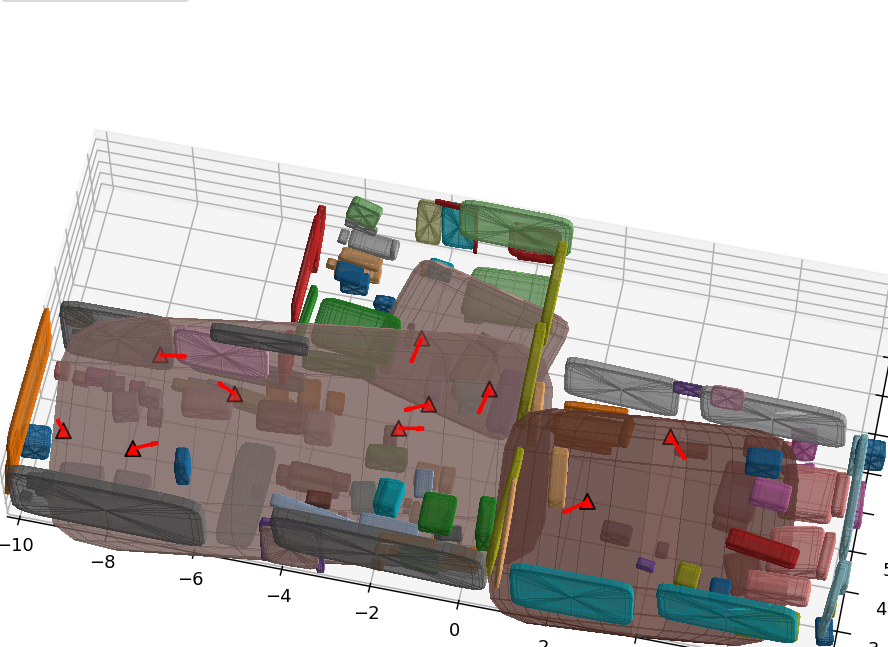
\includegraphics[width=\linewidth]{figures/superquadrics_3d_clean.png}
    \end{minipage}
    \vskip0.4ex
    \cpt{Figure 1: Super-quadric decomposition of a scene (189 primitives) with camera poses.}
  \end{psection}

  \flexgap

  \begin{psection}{Setup}
    \begin{itemize}
      \item \textbf{Dataset:} Aria Synthetic Environments (10 scenes)
      \item \textbf{Models:} VGGT for feed-forward poses (via MapAnything [2]),
            MASt3R for matching [3]; SuperDec [4] for the prior
      \item \textbf{Optimization:} full triangulation + surface BA in Ceres
    \end{itemize}
    \vskip0.4ex
    {\large
    \[
      E=\underbrace{\sum_{i,j}\rho\!\left(\lVert \pi(R_i,t_i,X_j)-x_{ij}\rVert^2\right)}_{\text{reprojection}}
       +\underbrace{\sum_{j}\Big(\lambda\,\lVert q_j\rVert\cdot\max\!\big(0,\,1-F(q_j)^{-\varepsilon_1}\big)\Big)^2}_{\text{one-sided surface prior}}
    \]}
    \vskip-0.2ex
    {\small where $F(\cdot)$ is the inside--outside function of the super-quadric
    $a(j)$ nearest to point $X_j$, $\varepsilon_1$ its shape parameter, and
    $\lambda$ the prior weight [5]. \textbf{Metric:} pose AUC@5$^\circ$.}
  \end{psection}

\end{minipage}
\end{column}
%---------------------------------------------------------------- RIGHT COLUMN
\begin{column}{\colwidth}
\begin{minipage}[t][\colheight][t]{\linewidth}

  \begin{psection}{Results}
    Three configurations: \textbf{VGGT-only} (feed-forward poses, AUC@5
    $=9.3$), \textbf{Baseline} (reprojection BA), and \textbf{Ours} (BA + the
    super-quadric prior). \textbf{The prior's benefit grows as the input gets
    sparser} --- the realistic relocalization regime.
    \vskip0.9ex
    \begin{center}
    \begin{minipage}{0.5\colwidth}
      \centering
      \begin{tikzpicture}
        \begin{axis}[posterchart,
          ybar, bar width=0.95cm, enlarge x limits=0.28,
          title={Pose AUC@5 vs.\ \# views},
          symbolic x coords={4,6,8}, xtick=data,
          xlabel={Number of input views}, ylabel={AUC@5 ($\%$)},
          ymin=0, ymax=48,
          nodes near coords, every node near coord/.append style={font=\small,/pgf/number format/.cd,fixed,fixed zerofill,precision=1},
          legend style={font=\normalsize,at={(0.5,1.18)},anchor=south,legend columns=2,draw=none,/tikz/every even column/.append style={column sep=6mm}},
          legend cell align=left,
        ]
          \addplot[fill=BarGray,draw=BarGray!70!black] coordinates {(4,39.3)(6,29.6)(8,27.9)};
          \addplot[fill=ETHBlue,draw=ETHBlue!70!black] coordinates {(4,40.7)(6,31.1)(8,28.0)};
          \legend{Baseline,Ours}
        \end{axis}
      \end{tikzpicture}\\[0.2ex]
      \cpt{Ours $\geq$ Baseline at every view count.}
    \end{minipage}\hfill
    \begin{minipage}{0.5\colwidth}
      \centering
      \begin{tikzpicture}
        \begin{axis}[posterchart,
          ybar, bar width=0.85cm, enlarge x limits=0.18,
          title={Gain from prior ($\Delta$AUC@5)},
          symbolic x coords={4,6,8,10}, xtick=data,
          xlabel={Number of input views}, ylabel={$\Delta$ AUC@5 (pp)},
          ymin=0, ymax=2.0,
          nodes near coords={\textbf{+\pgfmathprintnumber{\pgfplotspointmeta}}},
          every node near coord/.append style={font=\small,color=ETHBlueDark,/pgf/number format/.cd,fixed,precision=1},
        ]
          \addplot[fill=ETHBlue,draw=ETHBlue!70!black] coordinates {(4,1.3)(6,1.5)(8,0.1)(10,0.2)};
        \end{axis}
      \end{tikzpicture}\\[0.2ex]
      \cpt{$7\times$ larger at 6 views than at 10.}
    \end{minipage}
    \end{center}
    \vskip0.7ex
    \begin{beamercolorbox}[wd=\linewidth,sep=0.5cm,rounded=true,center]{block title}
      \large\bfseries\color{ETHBlueDark}
      +1.5 AUC@5 at 6 views ($\approx$5\% relative) vs.\ +0.2 at 10 views
    \end{beamercolorbox}
  \end{psection}

  \flexgap

  \begin{psection}{Discussion}
    At high view counts, dense multi-view correspondences already constrain the
    poses, so the prior is largely redundant ($+0.2$ at 10 views). As views drop
    and co-visibility collapses, reprojection alone under-constrains the geometry
    --- and the super-quadric surface fills exactly that gap, recovering up to
    $+2.0$ AUC@5 with light tuning at 4 views. ATE stays comparable throughout.
  \end{psection}

  \flexgap

  \begin{psection}{Conclusion}
    Transformer-based SfM cannot natively exploit an environment prior; we close
    this gap for relocalization. Encoding the prior as a super-quadric cloud and
    adding a point-to-quadric term to BA improves pose accuracy over both
    VGGT-only and standard BA --- most where it matters: \textbf{sparse,
    low-covisibility views}.
  \end{psection}

  \flexgap

  \begin{block}{References}
    {\small\setlength{\parindent}{0pt}\setlength{\emergencystretch}{3em}\raggedright\sloppy
    \noindent [1] Wang et al., \emph{VGGT: Visual Geometry Grounded Transformer}. CVPR 2025.\par
    \noindent [2] Keetha et al., \emph{MapAnything: Universal Feed-Forward Metric 3D Reconstruction}. 3DV 2026.\par
    \noindent [3] Leroy et al., \emph{Grounding Image Matching in 3D with MASt3R}. ECCV 2024.\par
    \noindent [4] Fedele et al., \emph{SuperDec: 3D Scene Decomposition with Superquadric Primitives}. ICCV 2025.\par
    \noindent [5] Mueller et al., \emph{Reconstructing People, Places, and Cameras}. CVPR 2025.\par}
  \end{block}

\end{minipage}
\end{column}
\end{columns}
\end{frame}
\end{document}
